\section{Phương pháp nghiên cứu}
\subsection{Linear Regression}
Nội dung.

% =========================================
\subsection{ARIMA}
Nội dung.

% =========================================
\subsection{RNN}
Nội dung. 

% =========================================
\subsection{LSTM}
Mạng bộ nhớ dài-ngắn (Long Short Term Memory networks), thường được gọi là LSTM - là một dạng đặc biệt của RNN, nó có khả năng học được các phụ thuộc xa. LSTM được giới thiệu bởi Hochreiter \& Schmidhuber (1997), và sau đó đã được cải tiến và phổ biến bởi rất nhiều người trong ngành. Chúng hoạt động cực kì hiệu quả trên nhiều bài toán khác nhau nên dần đã trở nên phổ biến như hiện nay.
\par
LSTM là một mạng nơ-ron tuần tự sâu trong học sâu, cho phép thông tin tồn tại lâu dài.
\par
Đây là một loại đặc biệt của Mạng Nơ-ron Tái Phát, có khả năng xử lý vấn đề vanishing gradient gặp phải bởi RNN.
    \indent\textbullet\ Output: \(c\), \(htct\), \(ht\). Ở đây, \(c\) biểu diễn trạng thái của ô (cell state) và \(h\) biểu diễn trạng thái ẩn (hidden state).
    \indent\textbullet\ Input: \(ct\)-1, \(ht\)-1\(ht\)-1, \(ht\)-1. Trong đó, \(xtxt\) là đầu vào tại trạng thái thứ \(t\) của mô hình. \(ct\)-1, \(ht\)-1\(ht\)-1, \(ht\)-1 là đầu ra từ lớp trước. \(h\) chơi vai trò tương tự như \(s\) trong RNN, trong khi \(c\) là điểm mới của LSTM.

\begin{minipage}{0.5\textwidth}
\centering
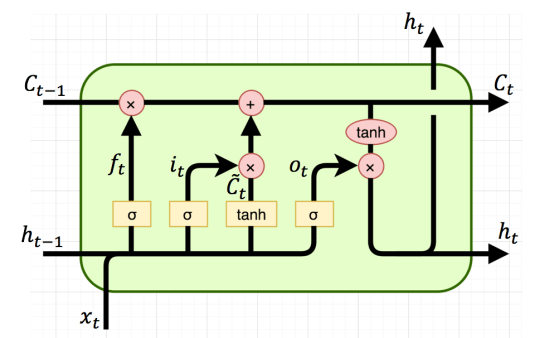
\includegraphics[width=1\textwidth]{resources/chapter-4/lstm-1.png}
\end{minipage}

Kí hiệu \(\sigma\), \(\tanh\) có nghĩa là dùng sigma, tanh và activation function
\par
\( f_t \), \( i_t \), \( o_t \) tương ứng với forget gate, input gate và output gate.\\
    \indent\textbullet\ Forget gate: \( f_t = \sigma\left(U_f \ast x_t + W_f \ast h_{t-1} + b_f\right) \)\\
    \indent\textbullet\ Input gate: \( i_t = \sigma\left(U_i \ast x_t + W_i \ast h_{t-1} + b_i\right) \)\\
    \indent\textbullet\ Output gate: \( o_t = \sigma\left(U_o \ast x_t + W_o \ast h_{t-1} + b_o\right) \)
\par
Nhận xét: \( 0 < f_t, i_t, o_t < 1 \); \( b_f, b_i, b_o \) là các hệ số bias.
\par
\( c_t = \tanh\left(U_c \ast x_t + W_c \ast h_{t-1} + b_c\right) \).
\par
\( c_t = f_t \ast c_{t-1} + i_t \ast c_t \), forget gate quyết định xem cần lấy bao nhiêu từ cell state trước và input gate sẽ quyết định lấy bao nhiêu từ input của state và hidden layer của layer trước.
\par
\( h_t = o_t \ast \tanh\left(c_t\right) \), output gate quyết định xem cần lấy bao nhiêu từ cell state để trở thành output của hidden state. Ngoài ra \( h_t \) cũng được dùng để tính ra output \( y_t \) cho state \( t \).


% =========================================
\subsection{GRU}
Nội dung.

% =========================================
\subsection{VARMA}
Nội dung. 

% =========================================
\subsection{Kalman Filter}
Nội dung.

% =========================================
\subsection{Meta-learning}
Meta-learning là một phương pháp trong học máy nhằm huấn luyện các mô hình để học một cách hiệu quả các nhiệm vụ mới với lượng dữ liệu hạn chế. Một trong những thuật toán nổi tiếng nhất trong meta-learning là Model-Agnostic Meta-Learning (MAML).
\par
\textbf{Model-Agnostic Meta-Learning (MAML)}
\par
Mục tiêu: MAML nhằm tìm một khởi tạo tốt cho các tham số của mô hình, giúp mô hình có thể được tinh chỉnh nhanh chóng trên một nhiệm vụ mới chỉ với một vài bước cập nhật gradient.
\par
\textbf{Khái niệm chính}
\par
    \indent\textbullet\ 1.	Phân phối nhiệm vụ (p(T)p(T)): Một phân phối trên các nhiệm vụ mà mô hình cần thích nghi.\\
    \indent\textbullet\ 2.	Mô hình cơ bản (\(f_\theta f_\theta\)): Mô hình được tham số hóa bởi \(\theta \theta\).\\
    \indent\textbullet\ 3.	Bộ dữ liệu hỗ trợ (Support Set): Bộ dữ liệu nhỏ từ đó mô hình học nhiệm vụ.\\
    \indent\textbullet\ 4.	Bộ dữ liệu truy vấn (Query Set): Bộ dữ liệu được dùng để đánh giá mô hình sau khi nó đã thích nghi với nhiệm vụ.\\
\par
\textbf{Các bước của thuật toán MAML}
\par
    \indent\textbullet\ 1.	Khởi tạo tham số mô hình: Bắt đầu với các tham số khởi tạo \(\theta \theta\).\\
    \indent\textbullet\ 2.	Lấy mẫu một loạt các nhiệm vụ: Lấy mẫu một loạt các nhiệm vụ {Ti}{Ti} từ phân phối nhiệm vụ p(T)p(T)\\
    \indent\textbullet\ 3. Đối với mỗi nhiệm vụ \(T_i\)\\
    	Lấy mẫu bộ dữ liệu hỗ trợ \(D_{T_i}^{\mathrm{train\ }}\) và bộ dữ liệu truy vấn \(D_{T_i}^{\mathrm{test\ }}\).\\ \\
     	Tính gradient của hàm mất mát trên bộ dữ liệu hỗ trợ với tham số \(\theta\):\\
            \[\nabla_\theta\mathcal{L}_{T_i}\left(f_\theta\right)\] \\
            Cập nhật các tham số sử dụng gradient:\\
            \[\theta_i^\prime=\theta-\alpha\nabla_\theta\mathcal{L}_{T_i}\left(f_\theta\right)\] \\
        \indent\textbullet\ 4. Cập nhật Meta\\
            Tính hàm mất mát trên bộ dữ liệu truy vấn sử dụng tham số đã cập nhật \(\theta_i^\prime\) \\ 
            \[\mathcal{L}_{T_i}\left(f_{\theta_i^\prime}\right)\]\\
            Tính gradient của hàm mất mát trên bộ dữ liệu truy vấn đối với các tham số khởi tạo \(\theta\) \\
            \[\nabla_\theta\mathcal{L}_{T_i}\left(f_{\theta_i^\prime}\right)\] \\
            Cập nhật các tham số khởi tạo \(\theta\) bằng cách trung bình các gradient qua loạt nhiệm vụ: \\
            \[\theta \gets \theta - \beta \sum_{i} \, \nabla_{\theta} \mathcal{L}_{T_{i}} \left( f_{\theta_{i}^{\prime}} \right)\]
            , với \(\beta\) là tốc độ học của meta.


% =========================================
\subsection{NBeats}
Nội dung.

% =========================================
\subsection{N-HiTS}
Nội dung.